% =============================================================
%  Thesis progress update, Accenture + Leiden supervisor
%  Author: Noah Bos
%  Date: 2026-06-01
%  Style: Accenture-inspired (purple #A100FF, sans-serif, clean)
%  Compile: pdflatex thesis_update_2026-06-01.tex   (run twice)
% =============================================================

\documentclass[aspectratio=169,11pt]{beamer}

% ---- Packages ----
\usepackage[T1]{fontenc}
\usepackage[utf8]{inputenc}
\usepackage{lmodern}
\usepackage{helvet}
\renewcommand{\familydefault}{\sfdefault}
\usepackage{xcolor}
\usepackage{tikz}
\usepackage{booktabs}
\usepackage{array}
\usepackage{tabularx}
\usepackage{calc}

% ---- Accenture palette ----
\definecolor{accpurple}{HTML}{A100FF}      % signature purple
\definecolor{accdark}{HTML}{1F1F1F}        % near-black text
\definecolor{accgray}{HTML}{6B6B6B}        % secondary text
\definecolor{accbg}{HTML}{F5F2FA}          % subtle purple wash
\definecolor{accaccent}{HTML}{460073}      % deep purple accent
\definecolor{accgreen}{HTML}{1AAF54}       % callout: good
\definecolor{accred}{HTML}{D6336C}         % callout: risk

% ---- Beamer setup: clean, no nav bars, frame number only ----
\setbeamertemplate{navigation symbols}{}
\setbeamertemplate{footline}{%
  \leavevmode%
  \hbox{%
    \begin{beamercolorbox}[wd=\paperwidth, ht=2.5ex, dp=1ex, right, rightskip=1.2em]{}%
      \color{accpurple}\scriptsize\insertframenumber{}\,/\,\inserttotalframenumber
    \end{beamercolorbox}}\vskip0pt%
}

\setbeamercolor{frametitle}{fg=accdark, bg=white}
\setbeamercolor{title}{fg=accdark}
\setbeamercolor{normal text}{fg=accdark, bg=white}
\setbeamercolor{itemize item}{fg=accpurple}
\setbeamercolor{itemize subitem}{fg=accpurple}
\setbeamercolor{itemize subsubitem}{fg=accpurple}
\setbeamercolor{enumerate item}{fg=accpurple}
\setbeamercolor{block title}{fg=white, bg=accpurple}
\setbeamercolor{block body}{fg=accdark, bg=accbg}
\setbeamercolor{alerted text}{fg=accred}

\setbeamerfont{frametitle}{size=\large, series=\bfseries}
\setbeamerfont{title}{size=\LARGE, series=\bfseries}
\setbeamerfont{subtitle}{size=\normalsize, series=\mdseries}

% Frame title with purple underline
\setbeamertemplate{frametitle}{%
  \vspace{0.8em}%
  \hspace{0.6em}\insertframetitle\\[-0.2em]%
  \hspace{0.6em}\textcolor{accpurple}{\rule{2.5em}{2pt}}\vspace{0.4em}%
}

\setbeamertemplate{itemize item}{\raisebox{0.3ex}{\scalebox{0.7}{\textcolor{accpurple}{$\blacksquare$}}}}
\setbeamertemplate{itemize subitem}{\raisebox{0.3ex}{\scalebox{0.6}{\textcolor{accpurple}{$\blacktriangleright$}}}}

% Custom title page
\defbeamertemplate*{title page}{accenture}{%
  \begin{tikzpicture}[remember picture, overlay]
    \fill[accpurple] (current page.north west) rectangle ([yshift=-1.3cm]current page.north east);
    \fill[accaccent] ([yshift=-1.3cm]current page.north west) rectangle ([yshift=-1.45cm]current page.north east);
  \end{tikzpicture}%
  \vspace{2.8cm}
  \begin{flushleft}
    \hspace{0.8em}{\color{accpurple}\rule{3em}{3pt}}\\[0.6em]
    \hspace{0.8em}{\usebeamerfont{title}\inserttitle}\\[0.4em]
    \hspace{0.8em}{\color{accgray}\usebeamerfont{subtitle}\insertsubtitle}\\[1.6em]
    \hspace{0.8em}{\color{accdark}\small\insertauthor}\\[0.2em]
    \hspace{0.8em}{\color{accgray}\footnotesize\insertdate}
  \end{flushleft}
}

% Inline coloured chip
\newcommand{\chip}[2]{\tikz[baseline=(c.base)]{\node[fill=#1!15, draw=#1, line width=0.4pt, rounded corners=2pt, inner sep=2pt, text=#1, font=\scriptsize\bfseries] (c) {#2};}}
\newcommand{\good}[1]{\chip{accgreen}{#1}}
\newcommand{\warn}[1]{\chip{accred}{#1}}
\newcommand{\info}[1]{\chip{accpurple}{#1}}

% =============================================================
%  TITLE
% =============================================================
\title{Explaining the Unexplained}
\subtitle{XAI faithfulness and stability on a continuously-updating airline propensity model}
\author{Noah Bos \textbar{} Accenture \textbar{} Leiden University thesis}
\date{1 June 2026}

\begin{document}

% ---------- Title ----------
\begin{frame}[plain, noframenumbering]
  \titlepage
\end{frame}

% ---------- Agenda ----------
\begin{frame}{Agenda}
  \vspace{0.3em}
  \begin{enumerate}
    \setlength\itemsep{0.6em}
    \item Research questions and scope
    \item \textbf{RQ1}, surrogate fidelity
    \item \textbf{RQ2}, explanation stability across splits
    \item \textbf{RQ3}, instability attribution
    \item \textbf{RQ4}, cross-offer replication
    \item Where the work stands, and what is left
  \end{enumerate}
  \vspace{0.8em}
  \begin{block}{Today}
    \footnotesize Focus is the full RQ1--RQ4 results pass. Writing the Discussion and Conclusion this week, submission \textbf{30 June}, defence \textbf{14 July}.
  \end{block}
\end{frame}

% =============================================================
%  RQs + SCOPE
% =============================================================
\begin{frame}{Four research questions}
  \begin{tabularx}{\linewidth}{@{}p{1.4em}X@{}}
    \textcolor{accpurple}{\textbf{RQ1}} & How accurately does the surrogate reproduce Pega's logged propensity scores on a held-out test set? \\[0.5em]
    \textcolor{accpurple}{\textbf{RQ2}} & How consistent are feature attribution rankings across temporal, route, and culture splits? \\[0.5em]
    \textcolor{accpurple}{\textbf{RQ3}} & When rankings shift, is the dominant source data drift ($\delta_d$), model churn ($\delta_m$), or explainer sensitivity ($\delta_e$)? \\[0.5em]
    \textcolor{accpurple}{\textbf{RQ4}} & Do the RQ1--RQ3 patterns replicate across three further offer variants with independently-updating Pega instances? \\
  \end{tabularx}
  \vspace{0.5em}
  \begin{block}{Scope}
    \footnotesize Luggage upsell, Email/Outbound channel. Primary variant: \textbf{L5B15} ($n=64{,}006$). Replication: \textbf{CLUG} (generic luggage), \textbf{BookingDotCom} (accommodation), \textbf{Cartrawler} (car rental), each governed by its own Pega ADM instance.
  \end{block}
\end{frame}

\begin{frame}{Why a CatBoost surrogate, and the two-layer pipeline}
  Pega ADM uses Naive Bayes internally and is queried offline only through logged $(\mathbf{X}_i, p_i)$ tuples. We train a surrogate $g \approx f$ on those scores; SHAP and LIME then explain $g$:
  \vspace{0.2em}
  \[
    f \;\longrightarrow\; g \;\longrightarrow\; \boldsymbol{\phi}(\mathbf{X})
  \]
  \vspace{-0.6em}
  \begin{itemize}
    \item \textbf{Five candidates compared} on the full fidelity suite (linear, GaussianNB, RF, LightGBM, CatBoost); CatBoost selected on $R^2$ + RMSE + $\tau_b$
    \item \textbf{TreeSHAP requires a tree model}, KernelSHAP on NB would $\sim$100$\times$ compute and add its own sampling variance
    \item \textbf{Native categorical + missing handling}, no arbitrary ordinal encoding as a confound
    \item \textbf{Depth 10} selected via Breiman's 1-SD rule (CV-max at depth 12; plateau across 10--13 confirms the optimum is inside the grid)
  \end{itemize}
\end{frame}

% =============================================================
%  RQ1: FIDELITY
% =============================================================
\begin{frame}{RQ1, surrogate fidelity across all four variants}
  \footnotesize
  \begin{tabular}{@{}l r r r r r@{}}
    \toprule
    \textbf{Variant}      & \textbf{$R^2$} & \textbf{Spearman $\rho$} & \textbf{Kendall $\tau_b$} & \textbf{RMSE}  & \textbf{$D_{KS}$} \\
    \midrule
    L5B15                 & 0.927          & 0.933                    & 0.785                     & 0.0026         & 0.087 \\
    CLUG                  & 0.954          & 0.920                    & 0.760                     & 0.0026         & 0.082 \\
    BookingDotCom         & 0.793          & 0.949                    & 0.811                     & 0.0002         & 0.064 \\
    Cartrawler            & 0.912          & \warn{0.615}             & 0.461                     & 0.0005         & 0.156 \\
    \bottomrule
  \end{tabular}

  \vspace{0.5em}
  \normalsize
  \begin{block}{Reading}
    \footnotesize Pointwise fit is strong on three of four variants. Cartrawler's low rank fidelity ($\rho = 0.615$) is carried forward as a caveat on its downstream attribution numbers. Moderate $D_{KS}$ across the board is expected: depth was selected on $\rho_S$, not a distributional criterion, and rank order is the operationally relevant property for Pega's scoring.
  \end{block}
\end{frame}

% =============================================================
%  RQ2: STABILITY
% =============================================================
\begin{frame}{RQ2, stability matrix on L5B15}
  Spearman $\rho_S$ on the full feature ranking across the five L5B15 splits:
  \vspace{0.2em}
  \scriptsize
  \renewcommand{\arraystretch}{0.95}
  \begin{tabular}{@{}l rrr rrr rrr@{}}
    \toprule
     & \multicolumn{3}{c}{\textbf{SHAP}} & \multicolumn{3}{c}{\textbf{LIME}} & \multicolumn{3}{c}{\textbf{Decision Tree}} \\
    \cmidrule(lr){2-4} \cmidrule(lr){5-7} \cmidrule(lr){8-10}
    Split & $\rho_S$ & $J_5$ & $J_{10}$ & $\rho_S$ & $J_5$ & $J_{10}$ & $\rho_S$ & $J_5$ & $J_{10}$ \\
    \midrule
    Temporal (early vs late) & 0.996 & 1.000 & 1.000 & 0.989 & 1.000 & 0.818 & 0.855 & 0.667 & 0.667 \\
    Route 1: ORY$\to$NCE vs ORY$\to$OPO & 0.994 & 1.000 & 1.000 & 0.986 & 0.667 & 0.818 & \warn{0.510} & 0.429 & 0.538 \\
    Route 2: ORY$\to$OPO vs NCE$\to$ORY & 0.990 & 1.000 & 0.818 & 0.858 & 1.000 & 0.818 & \warn{0.584} & 0.250 & 0.667 \\
    Route 3: NCE$\to$ORY vs TLS$\to$ORY & 0.987 & 0.667 & 0.818 & 0.992 & 1.000 & 1.000 & 0.817 & 0.667 & 0.667 \\
    Culture (fr-FR vs nl-NL) & 0.958 & 0.667 & 1.000 & 0.949 & 1.000 & 0.667 & \warn{0.666} & 0.429 & 0.667 \\
    \bottomrule
  \end{tabular}
  \vspace{0.5em}
  \normalsize
  \begin{block}{Pattern}
    \footnotesize \textbf{SHAP very stable everywhere} ($\rho_S \geq 0.958$). \textbf{LIME tracks SHAP closely}, with one dip on route pair 2. \textbf{DT collapses} on route and culture splits ($\rho_S$ down to 0.510). Bootstrap validation (10 re-fits, same data) confirms the DT gap on temporal, route 1, route 2, and culture is real signal, not fitting noise. Route 3 falls inside the bootstrap noise floor and is not interpreted as instability.
  \end{block}
\end{frame}

% =============================================================
%  RQ3: ATTRIBUTION
% =============================================================
\begin{frame}{RQ3, decomposing instability into its sources}
  \vspace{-0.2em}
  We decompose $\Delta\pi = 1 - \rho_S$ into three sources, monitored separately:
  \vspace{0.2em}
  \begin{columns}[T,onlytextwidth]
    \column{0.32\linewidth}
    \textbf{$\delta_d$, data drift}\\
    \scriptsize KS on propensity. Flagged if $\geq 0.10$.
    \column{0.32\linewidth}
    \textbf{$\delta_m$, model churn}\\
    \scriptsize Jaccard on active \texttt{modelVersion} IDs. Flagged if $\leq 0.10$.
    \column{0.32\linewidth}
    \textbf{$\delta_e$, explainer gap}\\
    \scriptsize $\rho_{\mathrm{SHAP}}-\rho_{\mathrm{DT}}$ (refit), $\rho_{\mathrm{SHAP}}-\rho_{\mathrm{LIME}}$ (sampling). Descriptive.
  \end{columns}

  \vspace{0.5em}
  \scriptsize
  \begin{tabular}{@{}l rrrr l@{}}
    \toprule
    \textbf{Split} & $\delta_d$ & $\delta_m$ & $\delta_e^{\mathrm{DT}}$ & $\delta_e^{\mathrm{LIME}}$ & \textbf{Source} \\
    \midrule
    L5B15 temporal              & 0.356 & 0.002 & 0.141 & 0.007  & Both \\
    Route 1 (ORY$\to$NCE vs ORY$\to$OPO) & 0.099 & 0.481 & 0.484 & 0.008  & \warn{Explainer} \\
    Route 2 (ORY$\to$OPO vs NCE$\to$ORY) & 0.094 & 0.547 & 0.406 & 0.132  & \warn{Explainer} \\
    Route 3 (NCE$\to$ORY vs TLS$\to$ORY) & 0.086 & 0.525 & 0.171 & $-0.005$ & \warn{Explainer} \\
    Culture (fr-FR vs nl-NL)    & 0.081 & 0.595 & 0.291 & 0.009  & \warn{Explainer} \\
    \bottomrule
  \end{tabular}

  \vspace{0.3em}
  \normalsize
  \begin{block}{Headline finding (RQ3)}
    \scriptsize On the same-window subgroup splits neither the data nor the model snapshots change, yet DT rankings differ substantially across them. \textbf{Under controlled conditions, the dominant source of observed instability is the explanation method itself.} SHAP is the most stable; LIME tracks SHAP closely (sampling variance is small).
  \end{block}
\end{frame}

% =============================================================
%  RQ4: REPLICATION
% =============================================================
\begin{frame}{RQ4 (i), temporal and route-pair replication}
  \vspace{-0.5em}
  \scriptsize
  \renewcommand{\arraystretch}{0.82}
  \begin{tabular}{@{}l rrrr l@{}}
    \toprule
    \textbf{Variant}                & $\delta_d$ & $\delta_m$ & $\delta_e^{\mathrm{DT}}$ & $\delta_e^{\mathrm{LIME}}$ & \textbf{Source} \\
    \midrule
    \multicolumn{6}{@{}l}{\textit{Temporal splits}} \\
    CLUG                            & 0.390 & 0.002 & 0.421 & 0.005    & Both \\
    BookingDotCom                   & 0.246 & 0.002 & 0.166 & 0.006    & Both \\
    Cartrawler                      & 0.721 & 0.002 & 0.373 & 0.025    & Both \\
    \midrule
    \multicolumn{6}{@{}l}{\textit{Route pair 1 (ORY$\to$NCE vs ORY$\to$OPO)}} \\
    CLUG                            & 0.052 & 0.406 & 0.363 & 0.015    & Explainer \\
    BookingDotCom                   & 0.116 & 0.416 & 0.711 & $-0.036$ & Dist.\ shift \\
    Cartrawler                      & 0.079 & 0.404 & 0.512 & 0.009    & Explainer \\
    \midrule
    \multicolumn{6}{@{}l}{\textit{Route pair 2 (ORY$\to$OPO vs NCE$\to$ORY)}} \\
    CLUG                            & 0.116 & 0.404 & 0.266 & 0.197    & Dist.\ shift \\
    BookingDotCom                   & 0.224 & 0.352 & 0.471 & $-0.024$ & Dist.\ shift \\
    Cartrawler                      & 0.059 & 0.361 & 0.757 & 0.367    & Explainer \\
    \midrule
    \multicolumn{6}{@{}l}{\textit{Route pair 3 (NCE$\to$ORY vs TLS$\to$ORY)}} \\
    CLUG                            & 0.069 & 0.426 & 0.490 & 0.015    & Explainer \\
    BookingDotCom                   & 0.062 & 0.396 & 0.333 & $-0.010$ & Explainer \\
    Cartrawler                      & 0.062 & 0.376 & 0.571 & 0.010    & Explainer \\
    \bottomrule
  \end{tabular}

  \vspace{0.4em}
  \footnotesize \textbf{Temporal} replicates fully (all $\rightarrow$ Both). \textbf{Routes} mostly replicate the L5B15 Explainer pattern; rows that flip to Dist.\ shift on borderline $\delta_d$ still carry the larger numerical contribution from $\delta_e^{\mathrm{DT}}$ (0.27--0.76).
\end{frame}

\begin{frame}{RQ4 (ii), culture split, the one place L5B15 does not replicate}
  \vspace{-0.3em}
  \footnotesize
  \begin{tabular}{@{}l rrrr l@{}}
    \toprule
    \textbf{Variant}                & $\delta_d$ & $\delta_m$ & $\delta_e^{\mathrm{DT}}$ & $\delta_e^{\mathrm{LIME}}$ & \textbf{Source} \\
    \midrule
    L5B15 (primary)                 & 0.081 & 0.595 & 0.291 & 0.009    & Explainer \\
    CLUG                            & 0.114 & 0.464 & 0.383 & $-0.017$ & Dist.\ shift \\
    BookingDotCom                   & 0.718 & 0.529 & 0.054 & $-0.060$ & Dist.\ shift \\
    Cartrawler                      & 0.689 & 0.564 & 0.177 & 0.352    & Dist.\ shift \\
    \bottomrule
  \end{tabular}

  \vspace{0.6em}
  \normalsize
  \begin{block}{Interpretation}
    \footnotesize L5B15's culture-driven propensity shift sits just below the threshold ($\delta_d = 0.081$); the three replication variants all cross it, with BookingDotCom and Cartrawler showing very large shifts ($\delta_d > 0.68$). Customer culture (FR vs NL) maps onto materially different propensity distributions for the cross-sell and third-party offers but not for the luggage upsell. \textbf{The methodological protocol generalises; the substantive role of any single feature dimension is product-context-specific.}
  \end{block}
\end{frame}

\begin{frame}{What SHAP says are the top features on L5B15}
  Top 10 features by mean absolute SHAP value, CatBoost surrogate:
  \begin{center}
    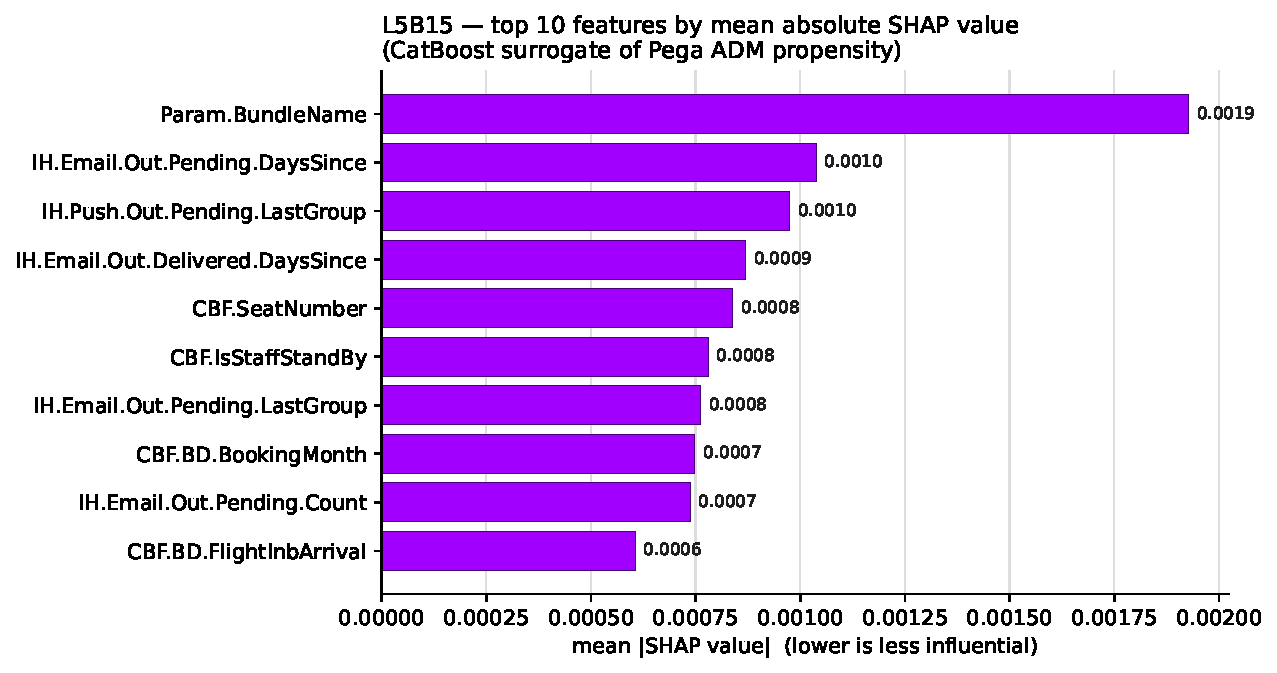
\includegraphics[width=0.85\linewidth]{figures/shap_top10_l5b15.pdf}
  \end{center}
\end{frame}

% =============================================================
%  WHERE THE WORK STANDS + TIMELINE
% =============================================================
\begin{frame}{Where the work stands, and what is left}
  \footnotesize
  \textbf{Done}
  \begin{itemize}
    \setlength\itemsep{0em}
    \item Data, methodology, RQ1--RQ4 results chapters written; tables and figures finalised
    \item Three-way instability attribution operationalised and replicated across four variants
    \item Sensitivity analyses in appendix: PSI bin count, Jaccard threshold, DT bootstrap, CV depth
  \end{itemize}
  \vspace{0.3em}
  \textbf{This week (1--7 June)}
  \begin{itemize}
    \setlength\itemsep{0em}
    \item Write the \textbf{Discussion} (link findings to the wider XAI literature, articulate limitations beyond what is already documented in Section 2.6)
    \item Write the \textbf{Conclusion} (summary of contributions + future directions)
  \end{itemize}
  \vspace{0.3em}
  \textbf{Timeline to defence}
  \begin{itemize}
    \setlength\itemsep{0em}
    \item 8--29 June, finalisation: full read-through, supervisor feedback round, polish
    \item \textbf{30 June} submission \quad $\bullet$ \quad \textbf{14 July} defence
  \end{itemize}
\end{frame}

\begin{frame}{Open questions for the supervisors}
  \begin{enumerate}
    \setlength\itemsep{0.8em}
    \item \textbf{Pega NB as a ``gold-label'' ranking?} Pega ADM exposes per-predictor importance directly via univariate NB likelihood contributions and bin lifts (Health Check predictor overview). Should we incorporate this as a reference ranking to validate the surrogate-based attributions, or stay strictly with the true black-box framing the methodology is built on?
    \item \textbf{Discussion scope}: how broadly should the discussion engage with the wider XAI literature given the single-airline setting, beyond the limitations already in Section~2.6?
    \item \textbf{Conclusion contributions}: keep the two-level framing (methodological protocol + empirical evidence under continuous online updating), or restructure?
  \end{enumerate}
\end{frame}

\begin{frame}[plain, noframenumbering]
  \begin{tikzpicture}[remember picture, overlay]
    \fill[accpurple] (current page.south west) rectangle (current page.north east);
  \end{tikzpicture}
  \vfill
  \begin{center}
    \color{white}{\fontsize{34}{38}\selectfont\textbf{Thank you}}\\[1em]
    \color{white}{\rule{4em}{2pt}}\\[1em]
    \color{white}{\normalsize Noah Bos \textbar{} noah.bos@accenture.com}
  \end{center}
  \vfill
\end{frame}

\end{document}
